\chapter{Visually Intuitive B Net apps}
\label{ch-bnet-apps}

The figures in this chapter were generated using
the free, open source app ``PyAgrum" (see Ref.\cite{pyagrum})


Whenever I introduce the subject of Bayesian Networks
to someone who has never seen them before, I recommend that the first thing they do is to
download a free bnet app from the internet such as PyAgrum\footnote{Alternative choices for bnet apps are Netica by www.norsys.com, or Hugin by www.hugin.com and several others.}, and play with it. It's a sure way of getting hooked
for life. That's how I got hooked, by an early bnet application called Ergo. As you can see from the pictures in this chapter,
the visual output generated by such applications is very ``explainable", intuitive and appealing.
  
In the late 1980's and early 1990's, partially fueled by the invention of
the junction tree algorithm (see Chapter \ref{ch-junc-tree}), there was much startup activity around Bnets. Bill Gates was a fan of them at that time, and he dedicated a lot of Microsoft manpower to do R\&D of bnets. The first version of Clippy and the first XBox recommender were in fact Bayesian Networks.

Here are a few of these addictive visuals generated by PyAgrum\footnote{``agrum" means citric fruit in French. }
for the simple diamond shaped  ``Wet Grass bnet".

To use PyAgrum, one first enters the input data consisting of the structure of the bnet and a TPM (Transition Probability Matrix)\footnote{A TPM is also called
a CPT, which stands for Conditional Probability Table}
for each node of the bnet.

When asked to display the input data, PyAgrum shows Fig.\ref{fig-wet-grass-bnet}.

When asked to ``infer" the probabilities of unobserved nodes $\rvr=Rain$
and $\rvw=WetGrass$,
assuming that as evidence, we observe that $\rvc=Cloudy=1$ and $\rvs=Sprinkler=1$, Pyagrum shows Fig.\ref{fig-wet-grass-evidence}.

\begin{figure}[h!]
\centering
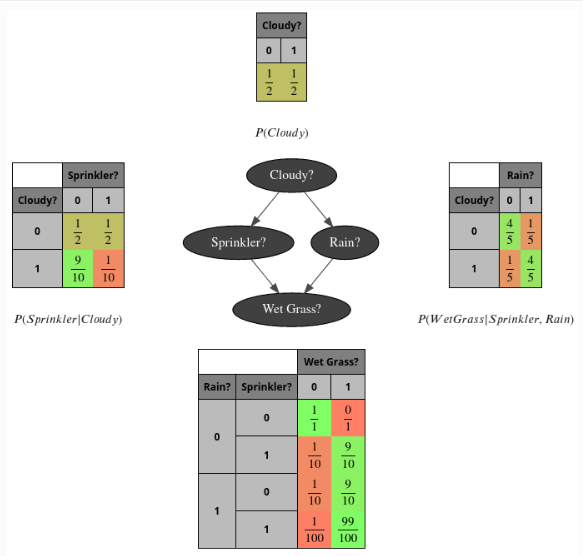
\includegraphics[width=5in]
{bnet-apps/wet-grass-bnet}
\caption{Structure (network, DAG) and a TPM for each node, of the ``Wet Grass" 
bnet.}
\label{fig-wet-grass-bnet}
\end{figure}

\begin{figure}[h!]
\centering
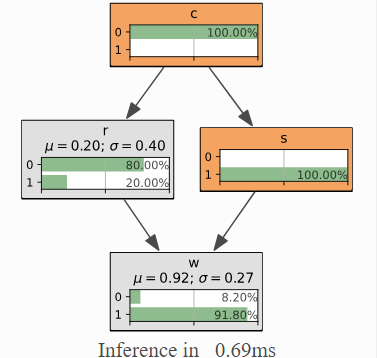
\includegraphics[width=4in]
{bnet-apps/wet-grass-evidence}
\caption{Probability histograms for every node of the Wet Grass bnet,
assuming that as evidence, we observe that $\rvc=Cloudy=1$ and $\rvs=Sprinkler=1$, i.e. the sprinkler was left ON and the day was not cloudy.}
\label{fig-wet-grass-evidence}
\end{figure}

PyAgrum can also  

\begin{itemize}

\item consider hard or soft evidence (or no evidence)
for each node. {\bf Hard evidence} means that only
one state of the node is observed whereas {\bf soft
evidence} means that each state of the node occurs with some probability.


\item calculate joint probability distributions and conditional joint probability distributions for multiple nodes of a bnet.
For example, it can calculate  $P(a,b|c,d)$ if $\rva, \rvb, \rvc, \rvd$ 
are 4  distinct nodes of the bnet.

\item calculate the strength of each arrow by calculating 
the mutual information between the two nodes defining the arrow.

\item find
the most likely value for each node. This is called the {\bf most probable explanation}.

\item calculate the Markov blanket for any node (See Chapter \ref{ch-mblanket})

\item draw influence diagrams and do associated calculations (see Chapter \ref{ch-inf-dia})

\item calculate conditional probabilities and adjustment formulae  that involve multiple do operators in the condition part. (see Chapter \ref{ch-do-calc})
\item do causal DAG discovery (what used to be called structure learning) (see Chapter \ref{ch-struc-learn})

\end{itemize}
and much more !

